\documentclass{article}

% if you need to pass options to natbib, use, e.g.:
% \PassOptionsToPackage{numbers, compress}{natbib}
% before loading nips_2017
%
% to avoid loading the natbib package, add option nonatbib:
% \usepackage[nonatbib]{nips_2017}

\usepackage[final]{nips_2017}

% to compile a camera-ready version, add the [final] option, e.g.:
% \usepackage[final]{nips_2017}

\usepackage[utf8]{inputenc} % allow utf-8 input
\usepackage[T1]{fontenc}    % use 8-bit T1 fonts
\usepackage{hyperref}       % hyperlinks
\usepackage{url}            % simple URL typesetting
\usepackage{booktabs}       % professional-quality tables
\usepackage{amsfonts}       % blackboard math symbols
\usepackage{nicefrac}       % compact symbols for 1/2, etc.
\usepackage{microtype}      % microtypography
\usepackage{graphicx}
\usepackage{natbib}

\graphicspath{{figures/}}

\title{Cracking Neural Network Hashes with Adversarial Examples}

% The \author macro works with any number of authors. There are two
% commands used to separate the names and addresses of multiple
% authors: \And and \AND.
%
% Using \And between authors leaves it to LaTeX to determine where to
% break the lines. Using \AND forces a line break at that point. So,
% if LaTeX puts 3 of 4 authors names on the first line, and the last
% on the second line, try using \AND instead of \And before the third
% author name.

\author{
  Conrad ~Christensen\\
  Deep Learning, Spring 2018\\
  New York University\\
  \href{mailto:conradbc@cims.nyu.edu}{\texttt{conradbc@cims.nyu.edu}} \\
  \And
  Da ~Ying\\
  Deep Learning, Spring 2018\\
  New York University\\
  \href{mailto:dy877@nyu.edu}{\texttt{dy877@nyu.edu}}
}

\begin{document}
% \nipsfinalcopy is no longer used

\maketitle

\begin{abstract}
    Success of neural networks have lead to a wide range of applications, some
    more appropriate than others. Due to a potential for parallelization, and
    ease of implementation, some works have suggested using neural networks as
    hash functions.  We believe this is a bad idea in terms of security, as
    neural networks are differentiable, which allows methods for collision
    search. We show that it is possible to generate hash collisions for some of
    the basic neural network hash functions. Additionally we explore the
    applicability of multiple techniques from adversarial example generation on
    generating collisions for a neural network hashing algorithm, comparing
    their efficacy.
\end{abstract}

\section{Introduction}
In computer security a cryptographic hash function is a function used to
reduced documents into a fixed size hash (often times represented by a
hexadecimal string).  The application for these range from download document
verification, to storage of passwords \cite{crypoHash}. One of the definiong
properties of this class of functions is that they are one-way. This means that
given a hash of a document, it is infeasible to find a document (a hash
collision) that produces the same hash (whether it is the same as the original
or not) \cite{crypoHash}.  This is particularly import if a company stores
password hashes. If these are lost to an adversary, it is important that the
adversary cannot find another password that produces the same hash, as then
they could use this to authenticate as one of the users.

There has been a recent increase in using machine learning to solve, or as part
of a solution, to systems problems. For example in \cite{learnedIndex}, the
authors use neural networks to learn the index distribution for data storage,
to replace B-Trees indexes for data retrieval. The problem of finding good
cryptographic using neural networks has also been proposed in multiple papers
\cite{hash1, hash2}. In this work we show that these hash functions
fundamentally do not satisfy the one-way requirement for cryptographic hashes,
as they expose sensitive information through the gradients of the network that
can be exploited to find hash collisions.

\section{Related Work}

Related to our approach of using the gradients of a neural network to alter
the input, is the work of finding adversarial examples that when fed to a
neural network, produce an unexpected output classification \cite{intriguing}.

This idea was first popularized in the work \cite{intriguing}; other methods
for generating these examples soon followed \cite{explaining}; and even defenses
for neural networks against being susceptible to these attacks emerged, such
as \cite{robust, ensemble, distil}. While effective to some degree, it was shown
in \cite{space} that adversarial examples exist in a large number of dimensions
of the input space, suggesting they may be a problem on a more fundamental 
level.

Neural network popularity has led to many unique uses for them. Some in already
solved domains. In \cite{hash1} an RNN is used to process data and produce
a fixed length hash value. This work measured the entropy of the hash function
by how many digits in the hash hexadecimal code were changed. Other authors,
including \cite{hash2} have also proposed using neural networks to create
one-way hash functions.

\section{Neural Hash Function}

The model that we will be attacking here, for the purpose of demonstrating
issues with neural network cryptographic hash functions, is that described in
\cite{hash1}.  Here we have a two-layer recurrent neural network (RNN) that
takes 512 bits as input, and produces 128 bit output through two linear
transformations with sigmoid activation functions. Weights of this network are
randomly initialized, but held constant there after to ensure the hash function
is deterministic. If there is another 512 bit block to read, this is
concatenated with the 128 bit output of the previous block, to produce another
128-bit output. 

See Figure \ref{fig:hashNN} for graphical representation of the hashing
process. It is worth noting that the neural network actually takes 640 bits
as input, where, for the first 512 bit block from the input file, the last
128 bits can be simply zeros. Once every block in the input is processed, the 
final 128 bit output is the hash for the input document.

%%% Separate image locations
%\begin{figure}[t]
    %\centering
    %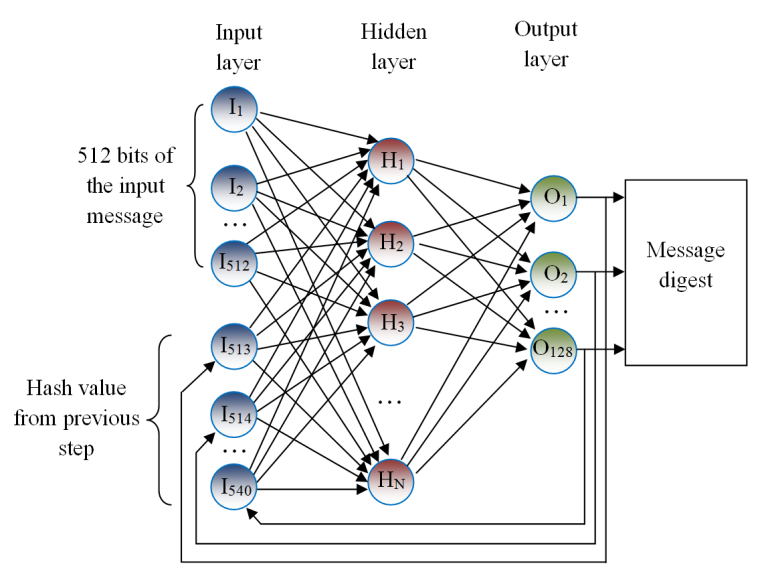
\includegraphics[width=90mm]{hash_nn_architecture}
    %\caption{A simple caption} 
    %\label{fig:hashNN}
%\end{figure}

%\begin{figure}[b]
    %\centering
    %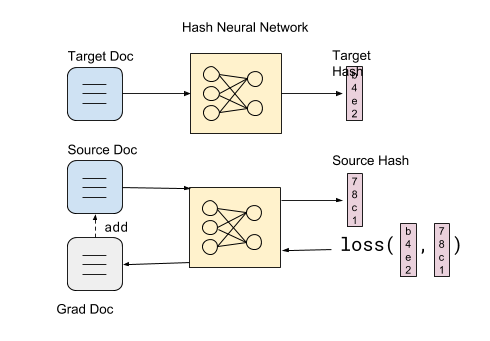
\includegraphics[width=90mm]{model_diagram}
    %\caption{Collision attack overview} 
    %\label{fig:model}
%\end{figure}


%%% Images side-by-side with minipages to save room.
\begin{figure}[t]
    \centering
    \begin{minipage}{.5\textwidth}
        \centering
        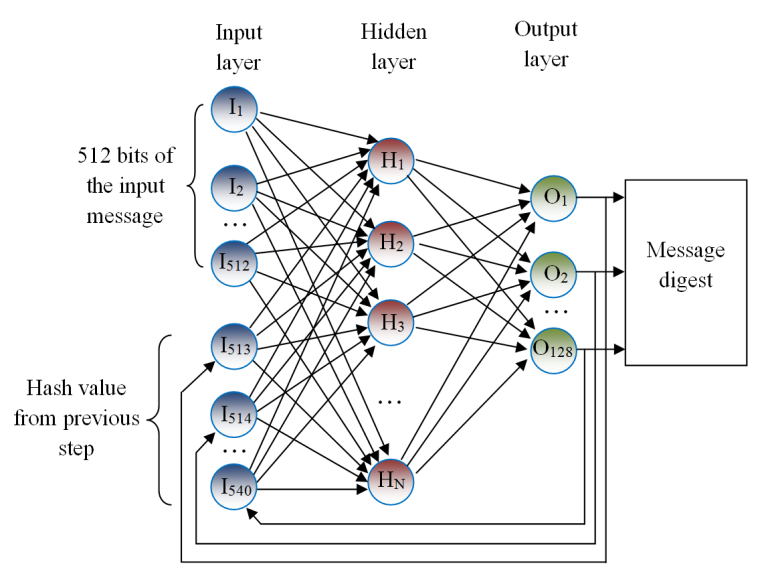
\includegraphics[width=\textwidth]{hash_nn_architecture}
        \caption{Hash function algorithm presented in \cite{hash1}}
        \label{fig:hashNN}
    \end{minipage}%
    \begin{minipage}{.5\textwidth}
        \centering
        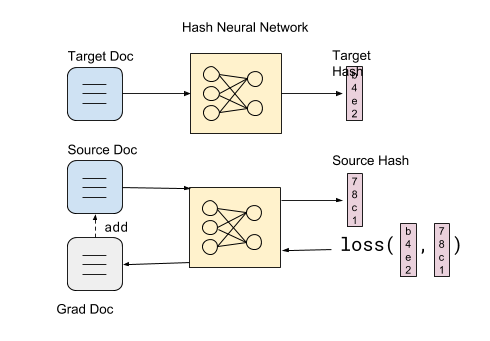
\includegraphics[width=\textwidth]{model_diagram}
        \caption{Collision attack overview} 
        \label{fig:model}
    \end{minipage}
\end{figure}


\section{Attack Approach}

Our attack approach starts with a target document, or just a target hash, to
find find a collision for. Given a target document, if there is one, the hash
is produced by feeding the document through the hash function described above.

Next, a start (or source) document is needed which will be converted into the
hash collision.  This can be arbitrary, or a specific document so that the
collision found will be somewhat similar to the source document. Here again we
can see a similarity with adversarial example generation, in that we would like
the collision found to be as close to the start document as possible (as an
adversarial is sought to be close to some valid input).

Then source document is fed into the hash neural network to produce a source hash.
This is then compared with the target hash in a loss function, to produce a loss
value of which to calculate the gradient. Here the mean squared error (MSE) loss
is used, bit wise between the target and source hash. An extra loss term is
added to keep the source input values close to one or zero (as they represent bits).
This loss is back-propagated until at the final layer the gradient of the loss
with respect to the input is acquired.

This calculated gradient of the source document is then added to the source
input, scaled by a learning rate. The new source document is then hashed again
to check if the hash value matches the target hash, else the gradient is
calculated again.  This model for finding a hash collision can be seen
graphically in Figure \ref{fig:model}.

\section{Results}
We evaluate the performance of our model, the success rate to generate pseudo-collisions and  the average time it takes. The first factor we take into consideration is the size of source file. Figures \ref{fig:docsize} shows the model achieves 100\% success rate when the size of source doc reaches 512 bytes. When size of source document is too small, the model lacks of information and value to change to reach the target hash, since our model does not add new value to the source document. It also shows the larger the source doc, the longer it takes to generate the collisions. When there is no restriction on choosing source documents, a documents with random 512 bytes gives the best performance.

Figure \ref{fig:lrate} shows the impact of learning rate on our model's performance. When our model cannot generate collisions within 1000 steps, it will be counted as a failure attempt. When learning rate is less than 1.0 or larger than 1.5, the model will have the risk of getting stuck in the local minimums, or failure to converge in time. The default learning rate is set to 1.

\subsection{Pseudo-collisions}
While our method is able to produce documents that hash to the target hash, these
aren't quite "true" collisions in that the source document contains values that
are not exactly 0 or 1. These values center around 0 and 1 but vary to some degree
to that the source document could not actually be written to disk as a string of 0's
and 1's without changing the source hash some. This is the reason for the added
loss term, which is $l'(r) = (r (r - 1))^2$, where $r$ is the source document
plus the gradient. This function  forms a 'w' with zero loss when $r = 0$ or
$r = 1$ and pushed the source document bits towards a valid value.

Controlling the above additional loss term is a regularization coefficient parameter, which decides how much the model wants to force the source documents bits towards a valid value. However, the difference on distribution of the final source documents value is minimal with different regularization coefficients, which can be seen in Figure \ref{fig:regcoeff}.

The regularization coefficient has minimal impact on performance when it is less then 0.01 which can be seen in Figure \ref{fig:regcoeff}. When regularization coefficient is too large, the model push the values of final source document to be really close to 0 or 1 with full force. It causes the model fail to converge. Figure \ref{fig:datadist} shows regularization coefficient does not make huge difference on the distribution of values of final source document.The coefficient does not have significant influence on average time to generate collisions. Therefore, as long as the coefficient is less than 0.01, the model will perform well.



%%% Images side-by-side with minipages to save room.
\begin{figure}[t]
    \centering
    \begin{minipage}{.45\textwidth}
        \centering
        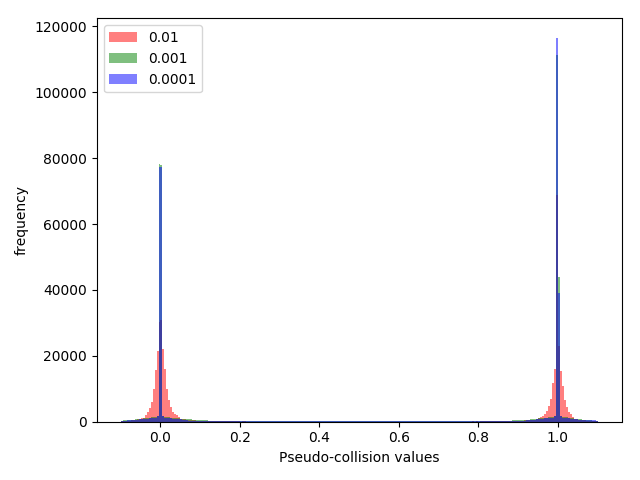
\includegraphics[width=\textwidth]{data_distribution}
        \caption{Pseudo-collisions value distribution with different regularization coefficient} 
        \label{fig:datadist}
    \end{minipage}%
    \hfill
    \begin{minipage}{.45\textwidth}
        \centering
        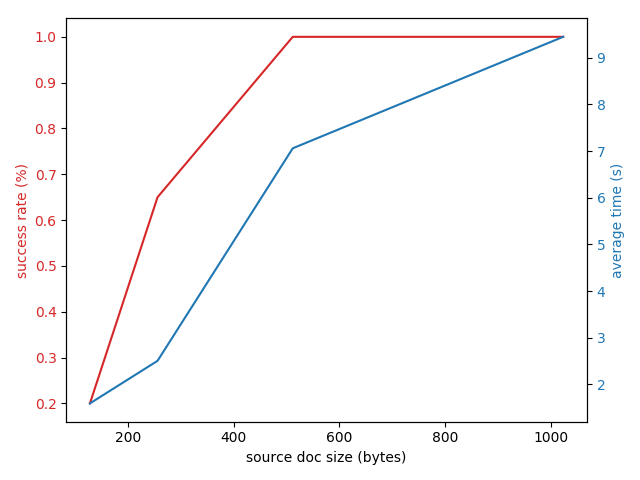
\includegraphics[width=\textwidth]{source_doc_size}
        \caption{Performance with different sizes of source docs}
        \label{fig:docsize}
    \end{minipage}
\end{figure}

\begin{figure}[t]
    \centering
    \begin{minipage}{.45\textwidth}
        \centering
        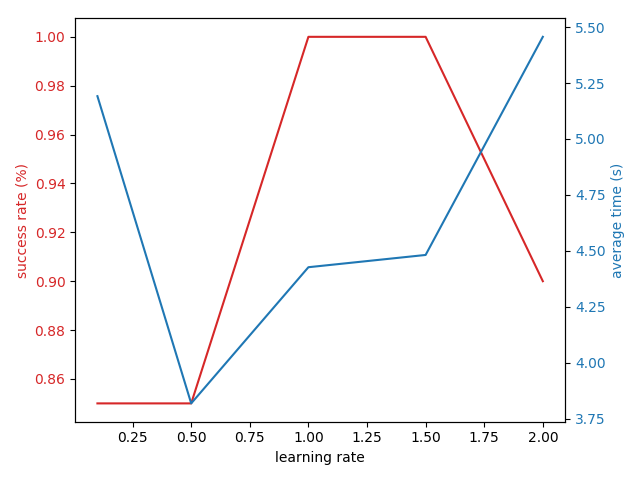
\includegraphics[width=\textwidth]{learning_rate}
        \caption{Performance with different learning rates} 
        \label{fig:lrate}    
    \end{minipage}%
    \hfill
    \begin{minipage}{.45\textwidth}
        \centering
        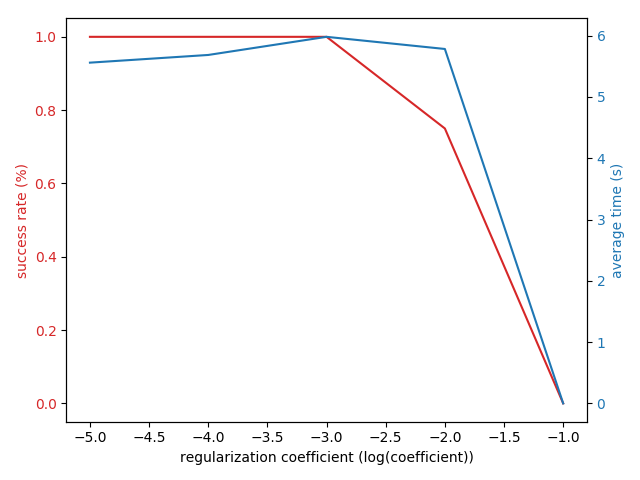
\includegraphics[width=\textwidth]{reg_coeff}
        \caption{Performance with different regularization coefficient}
        \label{fig:regcoeff}
    \end{minipage}
\end{figure}


\section{Conclusion}
We have demonstrated that neural network hash functions, at leas the one that
we targeted, are susceptible to attacks based on the information they expose in
their differentiability. While we were only able to generate pseudo-collisions,
we think it is more than possibly, with a little more though into the
additional loss term $l'$, to generate true hash collisions for this target
architecture. We also believe that other neural network hash functions will be
susceptible to similar attacks.

\bibliographystyle{unsrt}
\bibliography{ref} 

\end{document}
